\documentclass[11pt]{article}
\usepackage{url}
\usepackage{graphicx}

\begin{document}

\title{The NSF DataViz Hackathon for Polar CyberInfrastructure}
\author{Chris Mattmann}

\maketitle
\begin{abstract}
Add abstract here.
\end{abstract}


\section{Introduction}
The NSF DataViz Hackathon for Polar CyberInfrastructure was held at Parsons -- The New School for Design in New York City, New York on November 3-4, 2014. The meeting brought together cyberinfrastructure (CI) experts along with polar scientists from many career stages and data visualization experts including data artists to exploit the power of collaborative, face-to-face code development and interaction. 

The goals of the workshop were four-fold: (1) Produce code e.g., working prototypes using modern CyberInfrastructure technologies from the Apache Software Foundation, such as Apache Nutch (\url{http://nutch.apache.org/}), Apache Tika (\url{http://tika.apache.org/}) and Apache Solr (\url{http://lucene.apache.org/solr/}) and recommend CI technologies to the NSF Polar CyberInfrastructure program; (2) Create new Polar datasets e.g., reformatted from ASCII/CSV to modern JavaScript Object Notation, or JSON, geospatially locating datasets, loading datasets into search tools and Big Data infrastructure; (3) Design and evaluate new visualization approaches including D3.js (\url{http://d3.org/}), and TangeloHub (\url{https://github.com/tangelo-hub}); and (4) generate a final report summarizing the contributions and outcomes of the workshop. 

\begin{figure*}[htp]
    \centering
    \includegraphics[width=5in]{figs/fig1.png}
    \caption{The NSF DataViz Hackathon for Polar CyberInfrastructure website \protect\url{http://nsf-polar-cyberinfrastructure.github.io/datavis-hackathon/}}
    \label{fig:website}
\end{figure*}

\section{Sponsors and Organization}
The workshop was funded by Dr. Marco Tedesco and Dr. Daniel S. Katz of the U.S. National Science Foundation (NSF) and was also sponsored by cloud computing resources from Amazon Web Services (AWS) Inc., and Ms. Traci Ruthkoski. The workshop organization led by Dr. Chris Mattmann from the University of Southern California, and Parsons -- the New School and the Parsons School for Information Mapping (PIIM) and Mr. Jihoon Kang and Ms. Katie Wanner who hosted the meeting. Personnel from the Jet Propulsion Laboratory, California Institute of Technology (JPL) and the National Aeronautics and Space Administration (NASA) contributed to onsite logistics including creation of the website and the Earth Science Information Partners Federation (ESIP) provided cross promotion and marketing. The full attribution and contributors list to the workshop can be found at the following links \url{http://nsf-polar-cyberinfrastructure.github.io/datavis-hackathon/#committee} and \url{http://nsf-polar-cyberinfrastructure.github.io/datavis-hackathon/#contact}. 

% add organizing committee and participant breakdown here

\section{Participants and Data}
Forty total participants from twenty-eight institutions including academia, private industry, government and non governmental organizations participated in the meeting. Datasets were obtained in a variety of ways including: (1) using CyberInfrastructure to crawl NSFÕs Advanced Cooperative Arctic Data and Information System (ACADIS), NASA's Antarctic Master Directory (AMD and the National Snow and Ice Data Center's (NSIDC) Arctic Data Explorer (ADE));  (2) participants bringing their own data including station data from Ms. Carol Costanza of the University of Wisconsin Madison, Southern Ocean subsets of NASA's ECCO2 model outputs from Dr. Allen Pope of NSIDC, and Open Geospatial Consortium (OGC) web services by Dr. WenWen Li of Arizona State University. 

\begin{figure*}[htp]
    \centering
    \includegraphics[width=5in]{figs/fig2.png}
    \caption{Session proposer Dr. Lewis John McGibbney of NASA JPL gives a ``lightning talk'' describing his session {\em Polar Data Analytics as a service} \protect\url{https://github.com/NSF-Polar-Cyberinfrastructure/datavis-hackathon/issues/15} Meeting Room: The Orozco Room \protect\url{http://www.newschool.edu/leadership/provost/artcollection/new-school-murals/}}
    \label{fig:lightning}
\end{figure*}

% add statistics here

\section{Hackathon Organization}
Fifteen sessions total were `hacked on' over the two-day time-span and the participants in the meeting proposed all sessions and shaped the agenda leading up to, and during the meeting. The meeting agenda was run in a traditional "unconference" style. 

The unconference began with a `lightning talk' phase in which each session proposer stood up at the beginning of the workshop and gave a pitch for their session (proposed before the workshop), including a 1-2 minute brief synopsis and statement of expected outcomes. In the following time period, a coffee break, the hackathon participants identified their interest in attending a session by writing their name down on easels with session names and titles written down on paper. Workshop organizers then used this information to allocate sessions running in parallel alongside of four `hacks' over the two days. Each hack was a 1-2 hour time span of coding, discussion/sharing, preparing data, and creating visualizations that typically had between 3-5 sessions allocated to it. Data `artists' and visualization faculty from Parsons -- The New School and PIIM led by Mr. Aaron Hill provided design guidance and feedback to the participants by visiting selected sessions over the two day period.

\begin{figure*}[htp]
    \centering
    \includegraphics[width=5in]{figs/fig3.png}
    \caption{3-d printing model of Greenland ice thickness, bed elevation, and bathymetry from \protect\url{http://nsidc.org/data/nsidc-0092} contributed by Ms. Alex Boghosian, Lamont-Doherty Earth Observing Laboratory, Columbia University.}
    \label{fig:website}
\end{figure*}

\section{Outcomes}
Some notable outcomes of the sessions included: (1) a data converting script and web service to covert Antarctic Meteorology Research Center (AMRC) Automatic Weather Station (AWS) data from simple text data to JSON data and then to load that data into Apache Solr to create an AWS Polar data search (see more outcomes described in \url{https://github.com/NSF-Polar-Cyberinfrastructure/datavis-hackathon/issues/3}); (2) 3-d printing code for Arctic bathymetry and sea ice brine channels (read more about this session and its outcomes in \url{https://github.com/NSF-Polar-Cyberinfrastructure/datavis-hackathon/issues/50}); (3) a visualization wire-frame for a high school oriented tool to allow comparison of sea live rise using two glaciers as an example (see \url{https://github.com/NSF-Polar-Cyberinfrastructure/datavis-hackathon/issues/82} for more information); and (4) a prototype of a Tangelo web application.  The application combines imagery and dynamically-queried point information in an interactive web map.  Screenshots from the prototype are provided below in Figure 5.  The map in the browser displays the University of Wisconsin Automatic Weather Station (AWS) locations and NASA MODIS imagery. Imagery was added by querying NASA's WMS (Web Map Service) layer.  Dr. Curtis Lisle developed the Tangelo server architecture for AWS data and modified a sample OpenLayers application.  Mr. Justin Paul-Peters contributed the MODIS imagery datalayer.  Ms. Carol Costanza contributed by providing station source data and reference locations for debugging. Source code for the prototype is included in the hackathon repository, and described in  \url{https://github.com/NSF-Polar-Cyberinfrastructure/datavis-hackathon/issues/42}); 

\begin{figure*}[htp]
    \centering
    \includegraphics[width=5in]{figs/fig4.png}
    \caption{Wireframe of a glacier comparison tool showing the results of sea-level rise in the Arctic.}
    \label{fig:website}
\end{figure*}

\begin{figure*}[htp]
    \centering
    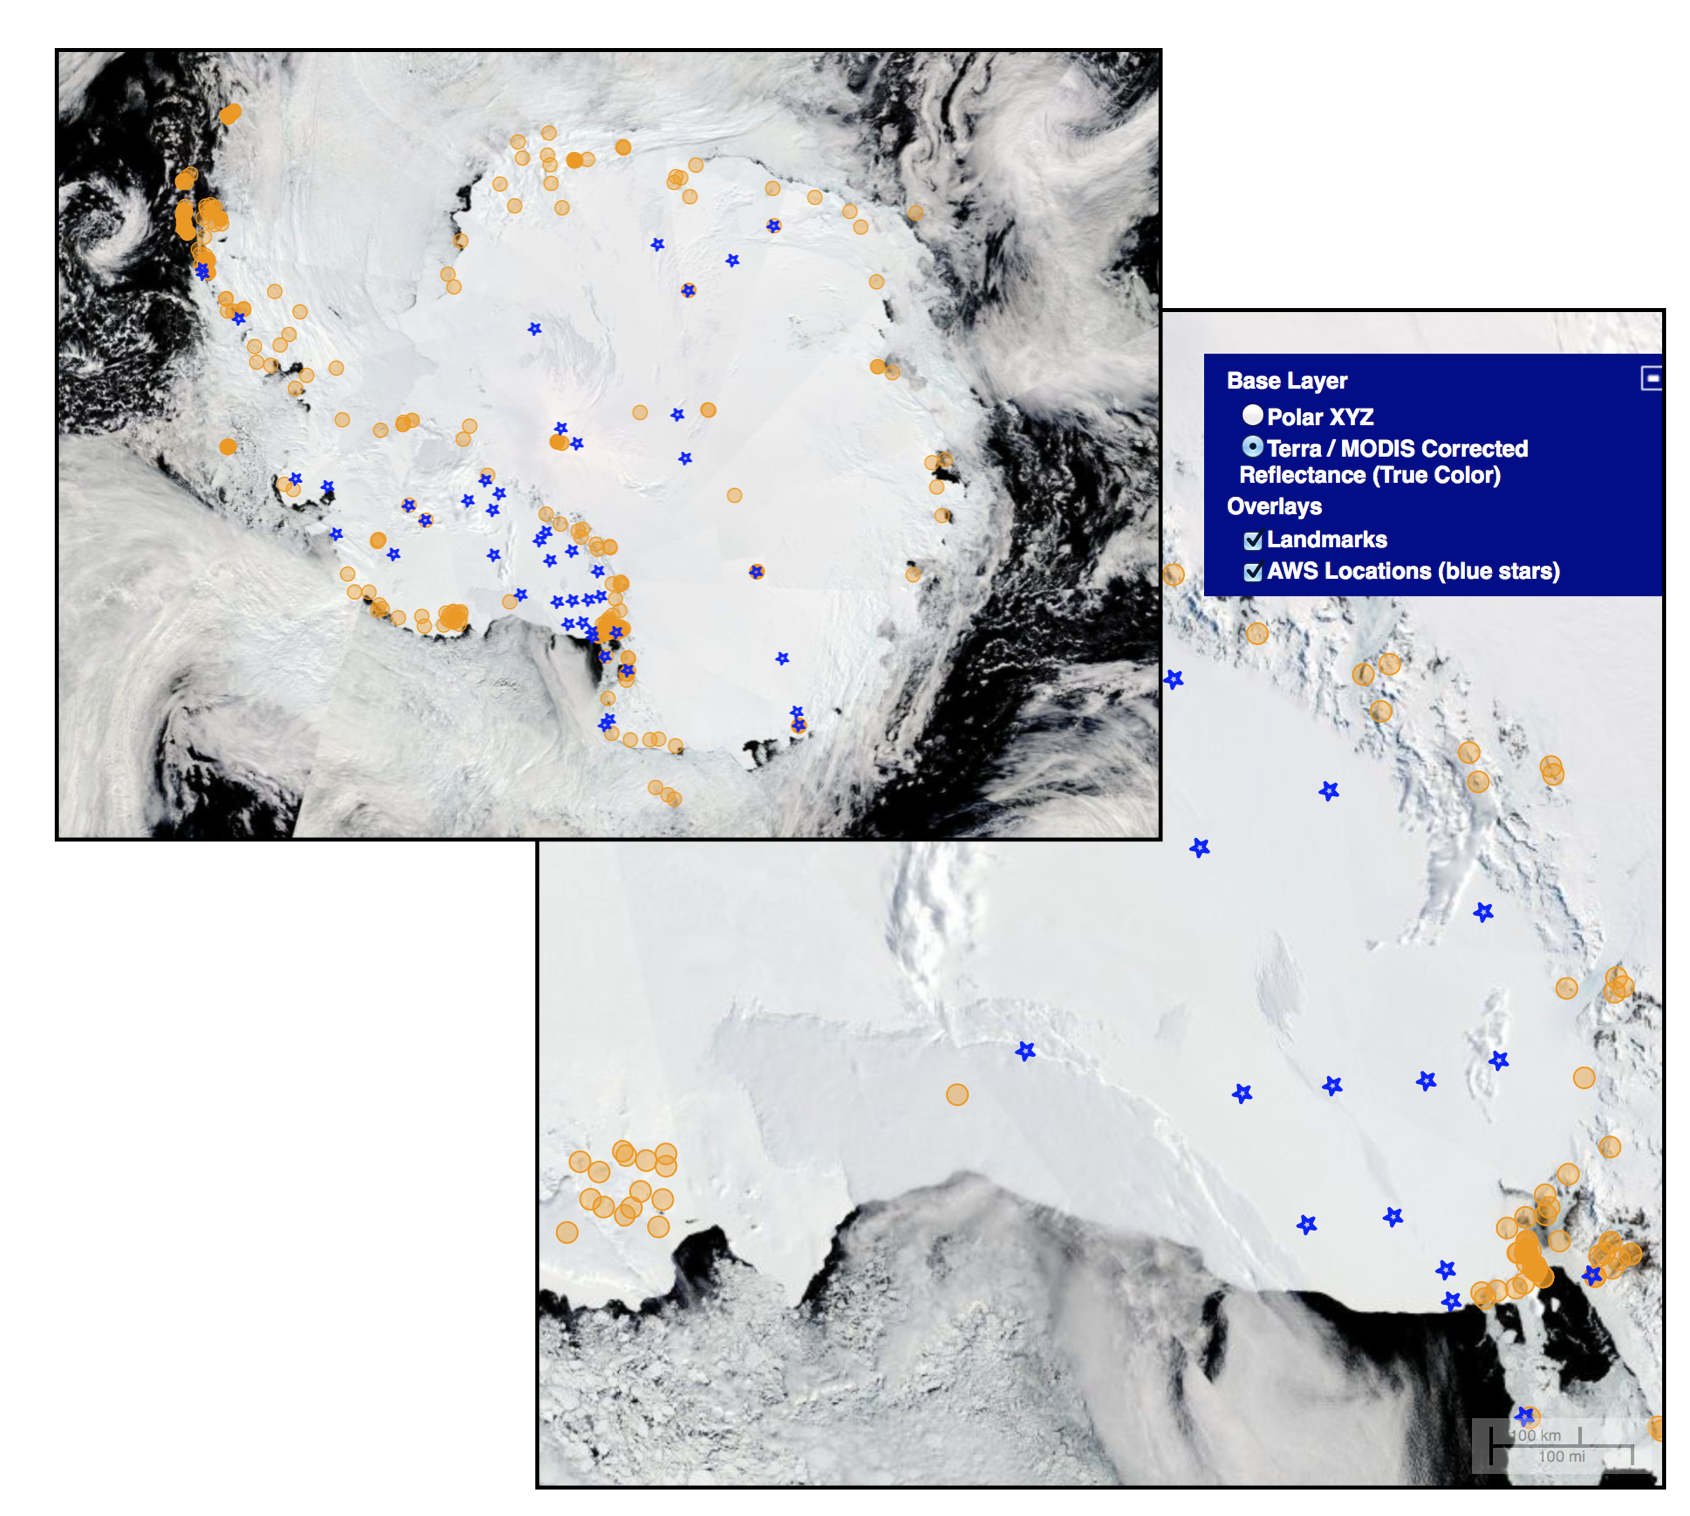
\includegraphics[width=5in]{figs/fig5.png}
    \caption{Screenshots from a Tangelo web map prototype that combines NASA polar imagery with dynamic AWS station layer (blue stars) and static reference points of interest (tan circles)}
    \label{fig:website}
\end{figure*}

All of the contributions from the workshop sessions are stored in a public Github repository freely accessible and licensed under the Apache License, version 2 (`ALv2') -- more information about the repository can be found at \url{https://github.com/NSF-Polar-Cyberinfrastructure/datavis-hackathon/}. 

\section{Recommendations}
%add recommendations
-AP: Some groups will be putting together proposals to build on Hackathon outcomes, and these should be supported to support the work and connections made
-AP: More direction in terms of pre-hackathin collaboration could lead to more concrete outcomes?
-AP: would be good to incorporate design at all levels of projects where possible, rather than intermittent consultation
-AP: i noticed there were sessions more "polar" and more CI; maybe require co-sponsors on sessions to get more crossover in the future?

\end{document}
